\chapter{Path planning}
% Change page numbers back to Arabic numerals and reset the page count
\label{cha:PathPlaning}

After we get the position information of car, obstacles, and boundary by image processing, if we want to hide and attack using laser, we really need to control car move from current position to expected position in a special space seeing Figure \ref{pathpoint},
For example, when we want to attack the opponent car behind the obstacles ,we need to catch up opponent car as soon as possible on the one hand, and on the another hand we should avoid the obstacles and boundary. But how to move car effectively in a special space is hard question. Robot path planning is used to find a collision-free sequence of motions (way point) between and an initial(current) position and a final(expected) position within a specified environment.

\begin{figure}[thb]
    \centering
    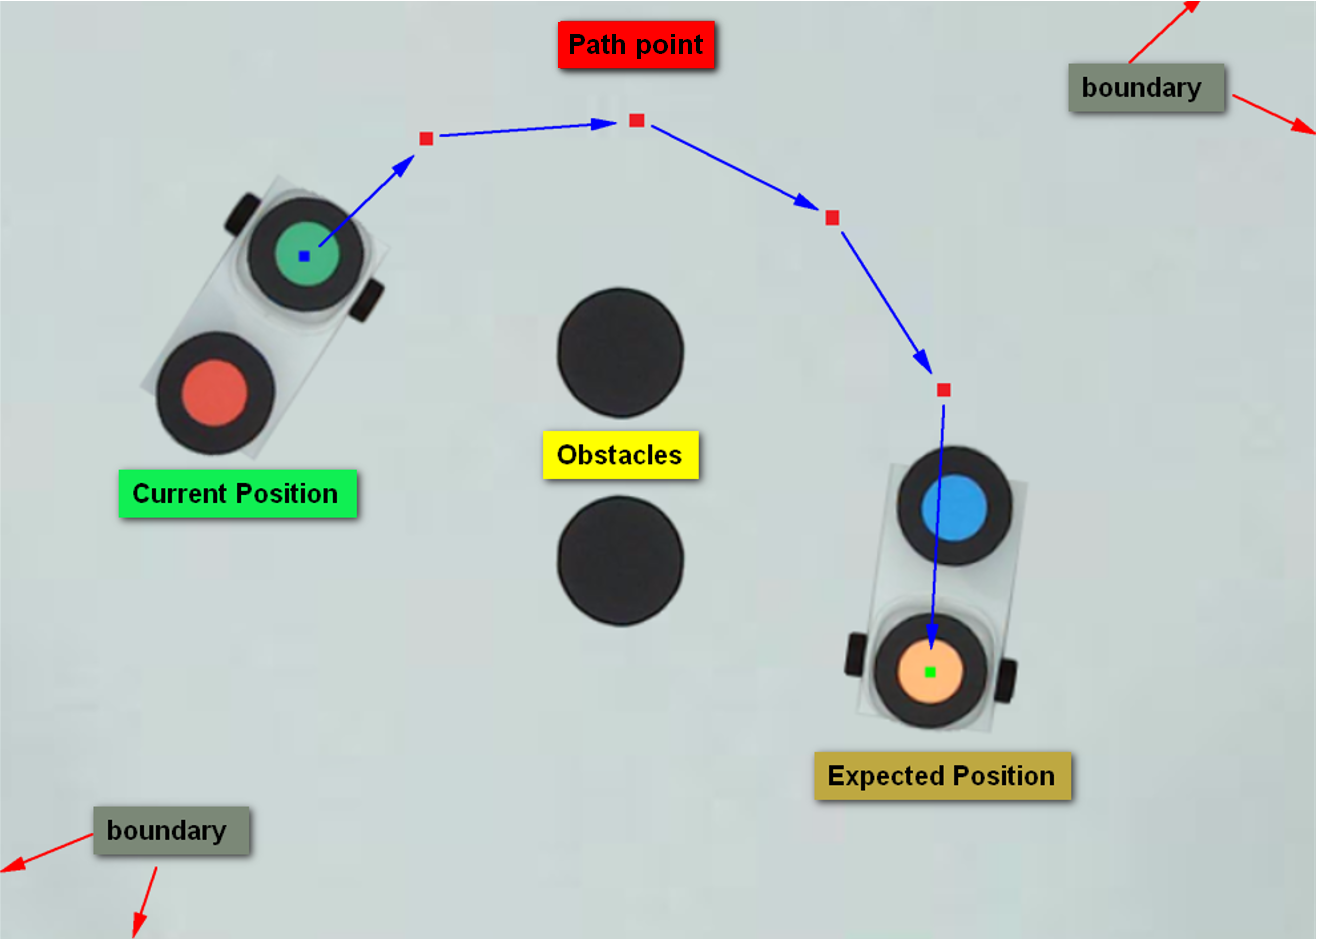
\includegraphics[width=1\textwidth]{images/PathPlaningPathPoint.png}
    \caption[How to find the path point]{How to find the path point.}\label{pathpoint}
\end{figure}

According to the special tasks and requirements of this project of MECH 6631 and after reading all kinds of path planning algorithms, a novel sampling and iterative based path planning algorithm (called Arc Sampling and Iterative Algorithm(ASIA)) is designed to used in this project.

\section{The principle and process of ASIA}

ASIA uses four steps to find and renew a new path point from current position to expected position.

\begin{enumerate}
    \item \textbf{Step 1: Get sampling points}\\
    As shown in Figure \ref{samplings}, First, we need to build a body coordinate system. The body coordinate origin is current position , and axis $X$ points the the expected position, and axis $Y$ and axis $X$ intersect at right angles. Second, initialize the value of sampling distance, sampling radian interval and total sampling radian. And get sampling sequence around current position.
    
    \begin{figure}[thb]
        \centering
        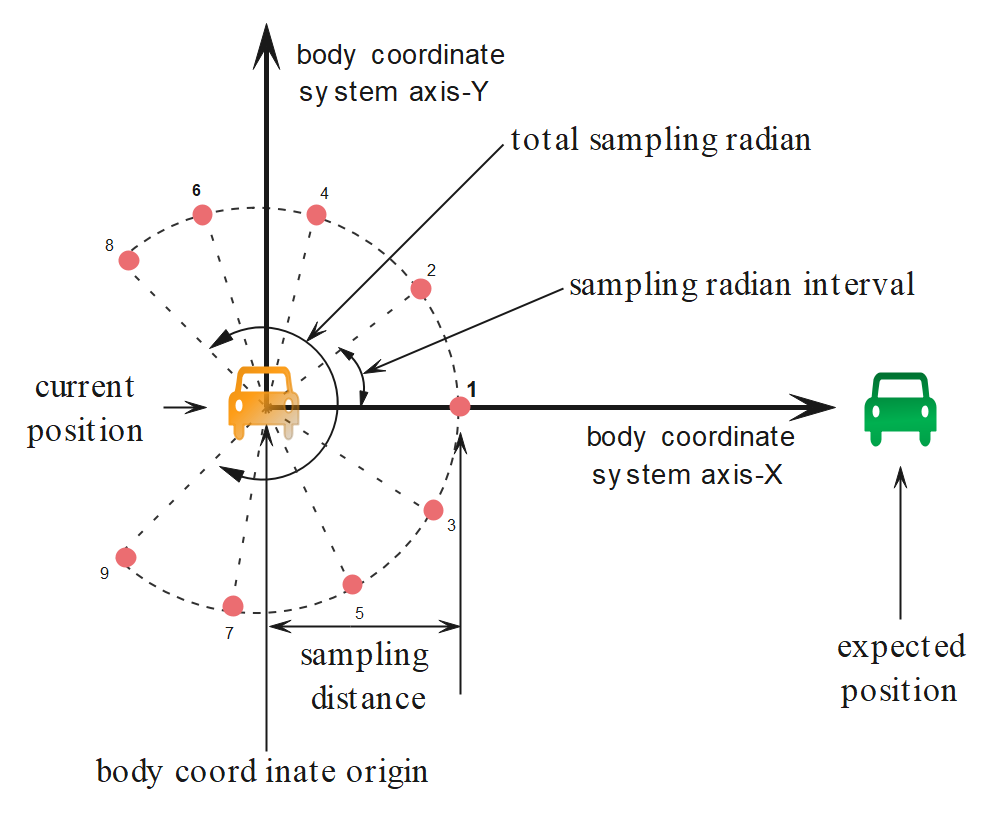
\includegraphics[width=1\textwidth]{images/PathPlaningSampling.png}
        \caption[How to find the path point]{How to get sampling points.}\label{samplings}
    \end{figure}
    
    \item \textbf{Step 2: Coordinate transformation}\\
    As seen in Figure \ref{transformation},We need to translate sampling points from body coordinate system to image coordinate system using rotation matrix after getting sampling points because we need to create path point sequence in image coordinate system.
    
    \begin{figure}[thb]
        \centering
        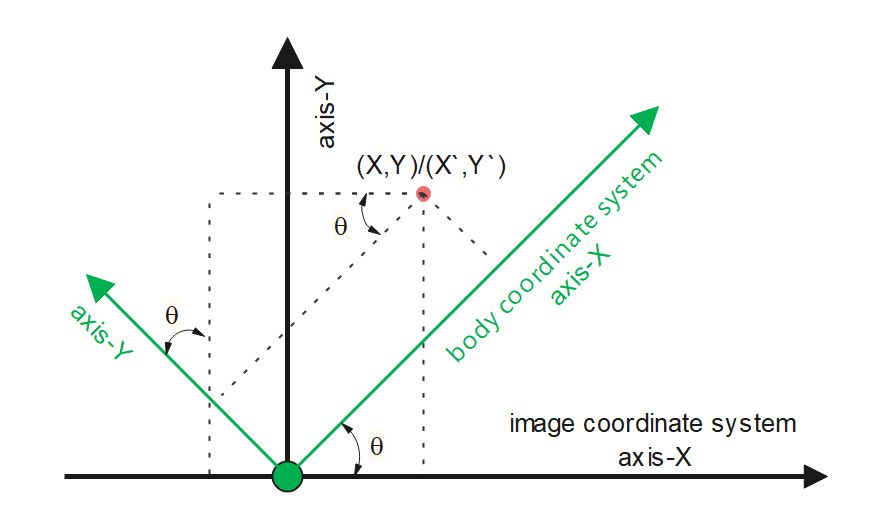
\includegraphics[width=1\textwidth]{images/PathPlaningRotationMarix.png}
        \caption[coordinate transformation]{coordinate transformation.}\label{transformation}
    \end{figure}
    
    According to the simple geometric knowledge in figure \ref{transformation}, we will get the transformation equation
    \begin{equation}
        \left\{\begin{matrix}
        X=X^{'}*cos\theta -Y^{'}*sin\theta\\Y=X^{'}*sin\theta +Y^{'}*cos\theta \label{con:rotation1}
        \end{matrix}\right.
    \end{equation}
    If the origin between body coordinate system and image coordinate system is not in the same position——in other words the origin position of body coordinate system is $(X_{0},Y_{0})$ in the mage coordinate system, a translation transform need to be added.
    
    \begin{equation}
    \begin{bmatrix}
    X \\Y
    \end{bmatrix}
    = 
    \begin{bmatrix}
    cos\theta & -sin\theta \\sin\theta & cos\theta
    \end{bmatrix} 
    \begin{bmatrix}
    X^{'}\\Y^{'}
    \end{bmatrix} 
    +\begin{bmatrix}
    X_{0}\\Y_{0}
    \end{bmatrix}  
    \end{equation}

    
    \item \textbf{Step 3: Get path point}\\
   As seen in Figure \ref{UpdatePathPoint},Judging if the sampling points(here it is represented by sampling points 1~9) is located in the free space sequentially (not coincide with the obstacle and is located within the image boundary). Once the conditions are met , the sampling point will be taken as the path point and renew current position, at the same time stop the judgement.
   
        \begin{figure}[thb]
        \centering
        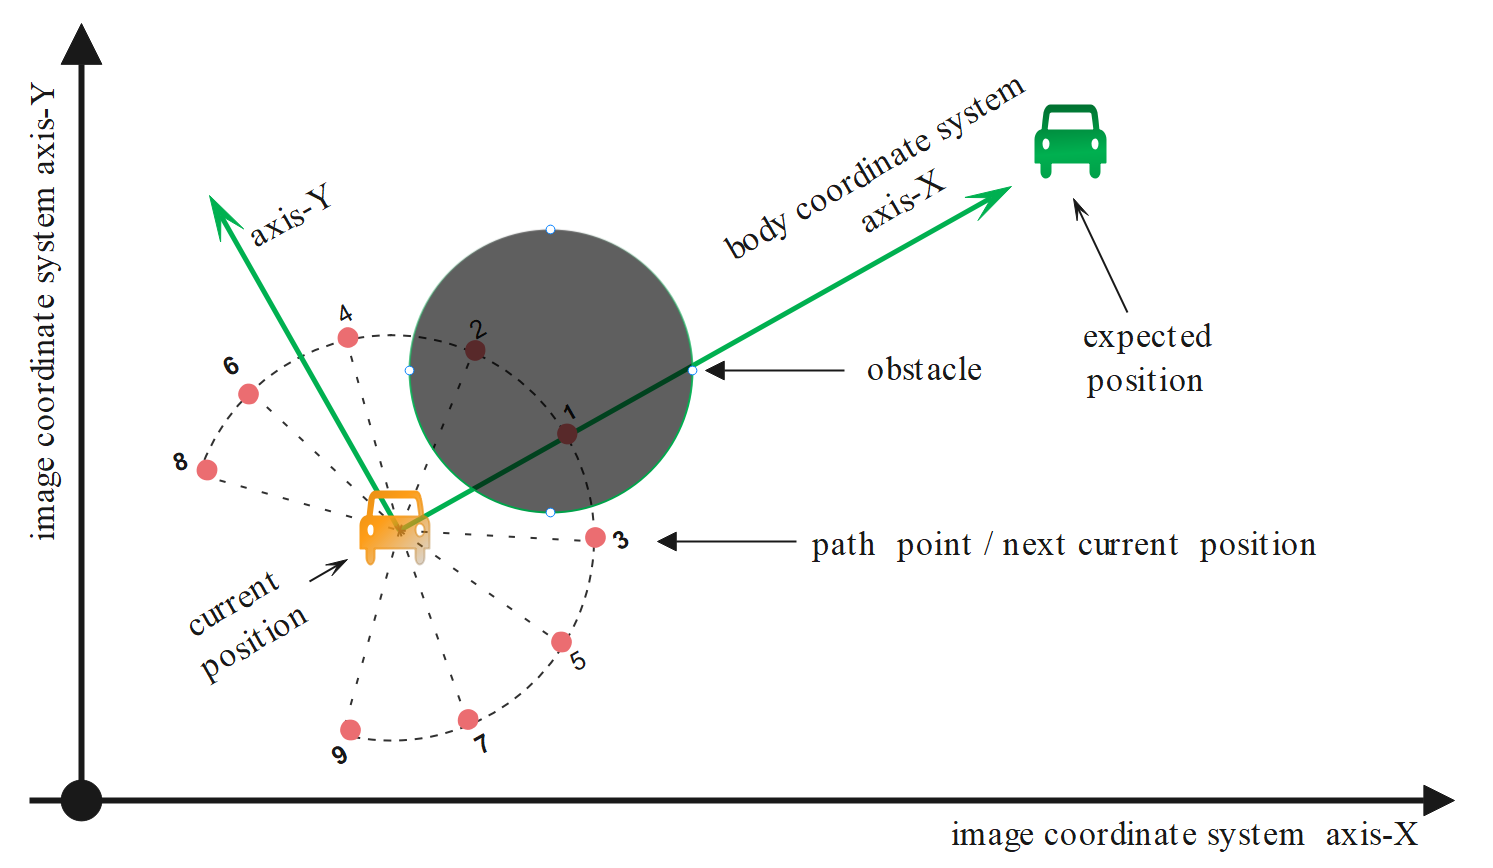
\includegraphics[width=1\textwidth]{images/PathPlaningUpdatePathPoint.png}
        \caption[how to get path point and renew current position]{how to get path point and renew current position.}\label{UpdatePathPoint}
    \end{figure}
    
    \item \textbf{Step 4: Iterate to get all of the path point}\\
    Iterate steps 1~3, until the distance between the current position and the expected position is less the the sampling distance. Up to now , we get all of the path point of path planing.
\end{enumerate}

\section{The implement of ASIA}

There are two parts codes to implement the ASIA. As seen in Figure \ref{part_1}, there are four Sub functions Sampling \underline{~} Array, Rotation \underline{~} Array(including TF \underline{~} X and TF \underline{~} Y), Get \underline{~} Angle \underline{~} Rotation and PathTrack to support ASIA.

    \begin{figure}[thb]
        \centering
        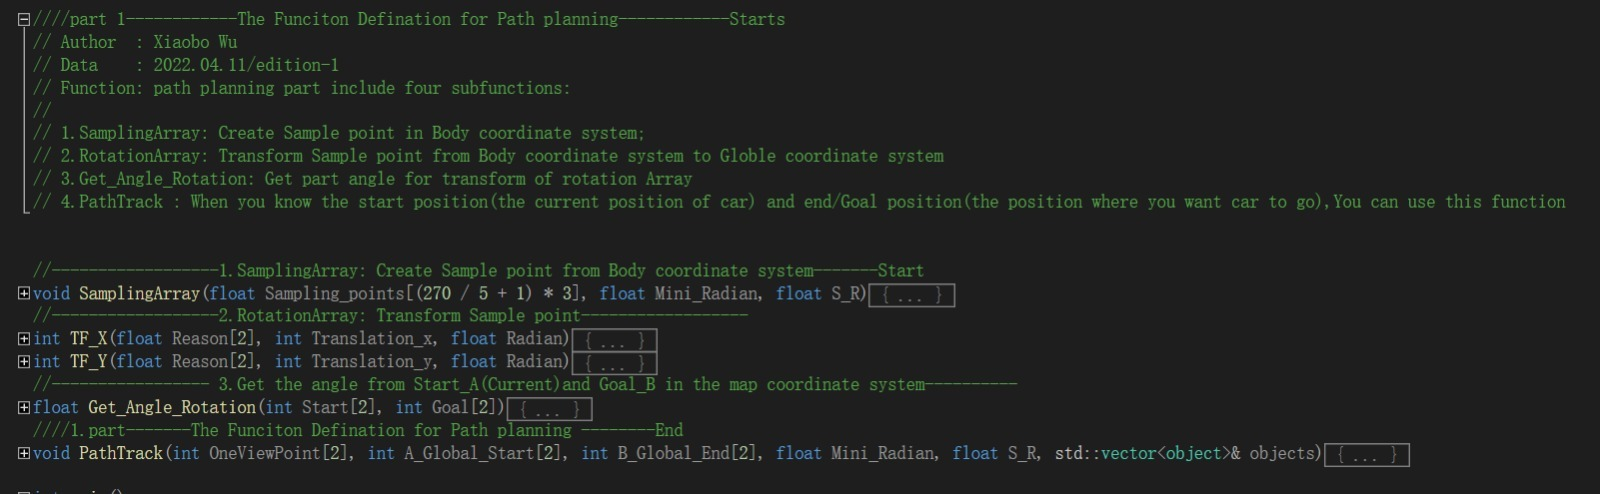
\includegraphics[width=1\textwidth]{images/part1.png}
        \caption[implement of ASIA Using four sub functions]{implement of ASIA Using four sub functions.}\label{part_1}
    \end{figure}
    

As seen in Figure \ref{part2}, Call the path planning / PathTrack, sub function in the main function.

    \begin{figure}[thb]
        \centering
        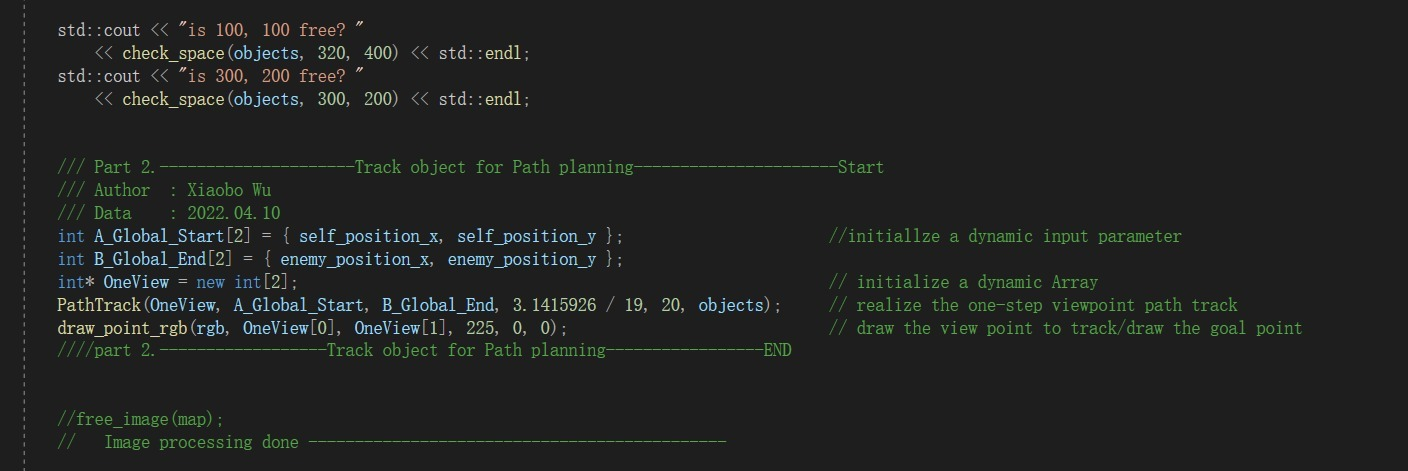
\includegraphics[width=1\textwidth]{images/part2.png}
        \caption[Call the path planning algorithm]{Call the path planning algorithm.}\label{part2}
    \end{figure}


